\documentclass[../Cover.tex]{subfiles}

\begin{document}

	\begin{minipage}[t][0.2\textheight][t]{0.1\textwidth} 
		\includegraphics[width=\textwidth]{\logoname}
	\end{minipage}
	\hfill
	\begin{minipage}[t][0.2\textheight][t]{0.8\textwidth}
		\begin{tabular}{ p{0.25\textwidth} l  }
			\\
			\textbf{React to Fire} \\
			\\[0.09\textheight]
		\end{tabular}
		\quad
		%%%%%%%%%%%%%%%%%%%%%%%%%%%
		% Quick Facts Table       %
		%%%%%%%%%%%%%%%%%%%%%%%%%%%
		\begin{tabular}{ | p{0.2\textwidth} | p{0.2\textwidth} | p{0.1\textwidth} |}
			\hline
			\rowcolor[HTML]{C0C0C0}\tiny Weapon Type & \tiny Distance & \tiny Par Time\\ 
			\hline
			\tiny Rifle/Carbine & \tiny 25yd& \tiny 4s \\ % EDIT HERE
			\hline
		\end{tabular}
	\end{minipage}
	%%%%%%%%%%%%%%%%%%%%%%%%%%%
	% Requirements      %
	%%%%%%%%%%%%%%%%%%%%%%%%%%%
	\begin{tabular}{p{0.25\textwidth}}
		\small Requirements \\
		\hline
		\tiny \begin{itemize} % EDIT HERE
			\item 2 IPSC targets, 5yd apart			
			\item Rounds Fired: 2 mags
			\item Starting Position: 90 degrees facing
		\end{itemize}		
		%%%%%%%%%%%%%%%%%
		% TikZ Diagrams %
		%%%%%%%%%%%%%%%%%		
		\begin{center}
			

\tikzset{every picture/.style={line width=0.75pt}} %set default line width to 0.75pt        

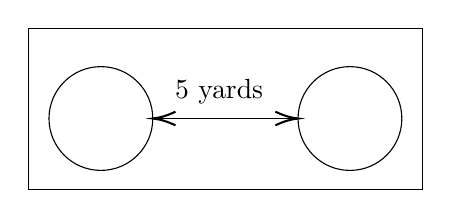
\begin{tikzpicture}[x=0.75pt,y=0.75pt,yscale=-1,xscale=1]
%uncomment if require: \path (0,235); %set diagram left start at 0, and has height of 235

%Shape: Circle [id:dp44350233650848403] 
\draw   (250,136) .. controls (250,122.19) and (261.19,111) .. (275,111) .. controls (288.81,111) and (300,122.19) .. (300,136) .. controls (300,149.81) and (288.81,161) .. (275,161) .. controls (261.19,161) and (250,149.81) .. (250,136) -- cycle ;
%Shape: Circle [id:dp7540662310947368] 
\draw   (370,136) .. controls (370,122.19) and (381.19,111) .. (395,111) .. controls (408.81,111) and (420,122.19) .. (420,136) .. controls (420,149.81) and (408.81,161) .. (395,161) .. controls (381.19,161) and (370,149.81) .. (370,136) -- cycle ;
%Straight Lines [id:da5895379960576028] 
\draw    (302,136) -- (368,136) ;
\draw [shift={(370,136)}, rotate = 180] [color={rgb, 255:red, 0; green, 0; blue, 0 }  ][line width=0.75]    (10.93,-3.29) .. controls (6.95,-1.4) and (3.31,-0.3) .. (0,0) .. controls (3.31,0.3) and (6.95,1.4) .. (10.93,3.29)   ;
\draw [shift={(300,136)}, rotate = 0] [color={rgb, 255:red, 0; green, 0; blue, 0 }  ][line width=0.75]    (10.93,-3.29) .. controls (6.95,-1.4) and (3.31,-0.3) .. (0,0) .. controls (3.31,0.3) and (6.95,1.4) .. (10.93,3.29)   ;
%Shape: Rectangle [id:dp0919307770262141] 
\draw   (240,92.5) -- (430,92.5) -- (430,170) -- (240,170) -- cycle ;


% Text Node
\draw (332,123) node   [align=left] {5 yards};


\end{tikzpicture}

		\end{center}		
		\\[0.6\textheight]
	\end{tabular}
	% Steps and Scoring	
	\begin{tabular}{ | p{0.65\textwidth} |}
		\hline
		%%%%%%%%%%%%%%%%%%%%%%%%%%%
		% Steps                   %
		%%%%%%%%%%%%%%%%%%%%%%%%%%%
		\rowcolor[HTML]{C0C0C0}Steps\\ 
		\hline
		\tiny \begin{enumerate}[topsep=0pt, partopsep=0pt]
			\item  Begin facing 90deg left or right from target at a distance of 25 yds
			\item On go, turn to face target 1, raise weapon, fire twice at target 1
			\item Drop to kneel, perform combat reload
			\item From kneeling, fire twice at target 2
		\end{enumerate}		
		\\ [0.25\textheight]
		\hline
		%%%%%%%%%%%%%%%%%%%%%%%%%%%
		% Scoring                 %
		%%%%%%%%%%%%%%%%%%%%%%%%%%%
		\rowcolor[HTML]{C0C0C0}Scoring \\
		\hline
		\tiny \begin{itemize}[topsep=0pt, partopsep=0pt]
			\item one % EDIT HERE
			\item Passing Hit Factor HF): 
		\end{itemize}		
		\\ [0.25\textheight]
		\hline
	\end{tabular}
\end{document}
